% Options for packages loaded elsewhere
\PassOptionsToPackage{unicode}{hyperref}
\PassOptionsToPackage{hyphens}{url}
%
\documentclass[
]{article}
\usepackage{amsmath,amssymb}
\usepackage{lmodern}
\usepackage{iftex}
\ifPDFTeX
  \usepackage[T1]{fontenc}
  \usepackage[utf8]{inputenc}
  \usepackage{textcomp} % provide euro and other symbols
\else % if luatex or xetex
  \usepackage{unicode-math}
  \defaultfontfeatures{Scale=MatchLowercase}
  \defaultfontfeatures[\rmfamily]{Ligatures=TeX,Scale=1}
\fi
% Use upquote if available, for straight quotes in verbatim environments
\IfFileExists{upquote.sty}{\usepackage{upquote}}{}
\IfFileExists{microtype.sty}{% use microtype if available
  \usepackage[]{microtype}
  \UseMicrotypeSet[protrusion]{basicmath} % disable protrusion for tt fonts
}{}
\makeatletter
\@ifundefined{KOMAClassName}{% if non-KOMA class
  \IfFileExists{parskip.sty}{%
    \usepackage{parskip}
  }{% else
    \setlength{\parindent}{0pt}
    \setlength{\parskip}{6pt plus 2pt minus 1pt}}
}{% if KOMA class
  \KOMAoptions{parskip=half}}
\makeatother
\usepackage{xcolor}
\IfFileExists{xurl.sty}{\usepackage{xurl}}{} % add URL line breaks if available
\IfFileExists{bookmark.sty}{\usepackage{bookmark}}{\usepackage{hyperref}}
\hypersetup{
  pdftitle={退出に関する pooled logit QMLE DiD 推定図},
  pdfauthor={Ayumu Tanaka},
  hidelinks,
  pdfcreator={LaTeX via pandoc}}
\urlstyle{same} % disable monospaced font for URLs
\usepackage[margin=1in]{geometry}
\usepackage{color}
\usepackage{fancyvrb}
\newcommand{\VerbBar}{|}
\newcommand{\VERB}{\Verb[commandchars=\\\{\}]}
\DefineVerbatimEnvironment{Highlighting}{Verbatim}{commandchars=\\\{\}}
% Add ',fontsize=\small' for more characters per line
\usepackage{framed}
\definecolor{shadecolor}{RGB}{248,248,248}
\newenvironment{Shaded}{\begin{snugshade}}{\end{snugshade}}
\newcommand{\AlertTok}[1]{\textcolor[rgb]{0.94,0.16,0.16}{#1}}
\newcommand{\AnnotationTok}[1]{\textcolor[rgb]{0.56,0.35,0.01}{\textbf{\textit{#1}}}}
\newcommand{\AttributeTok}[1]{\textcolor[rgb]{0.77,0.63,0.00}{#1}}
\newcommand{\BaseNTok}[1]{\textcolor[rgb]{0.00,0.00,0.81}{#1}}
\newcommand{\BuiltInTok}[1]{#1}
\newcommand{\CharTok}[1]{\textcolor[rgb]{0.31,0.60,0.02}{#1}}
\newcommand{\CommentTok}[1]{\textcolor[rgb]{0.56,0.35,0.01}{\textit{#1}}}
\newcommand{\CommentVarTok}[1]{\textcolor[rgb]{0.56,0.35,0.01}{\textbf{\textit{#1}}}}
\newcommand{\ConstantTok}[1]{\textcolor[rgb]{0.00,0.00,0.00}{#1}}
\newcommand{\ControlFlowTok}[1]{\textcolor[rgb]{0.13,0.29,0.53}{\textbf{#1}}}
\newcommand{\DataTypeTok}[1]{\textcolor[rgb]{0.13,0.29,0.53}{#1}}
\newcommand{\DecValTok}[1]{\textcolor[rgb]{0.00,0.00,0.81}{#1}}
\newcommand{\DocumentationTok}[1]{\textcolor[rgb]{0.56,0.35,0.01}{\textbf{\textit{#1}}}}
\newcommand{\ErrorTok}[1]{\textcolor[rgb]{0.64,0.00,0.00}{\textbf{#1}}}
\newcommand{\ExtensionTok}[1]{#1}
\newcommand{\FloatTok}[1]{\textcolor[rgb]{0.00,0.00,0.81}{#1}}
\newcommand{\FunctionTok}[1]{\textcolor[rgb]{0.00,0.00,0.00}{#1}}
\newcommand{\ImportTok}[1]{#1}
\newcommand{\InformationTok}[1]{\textcolor[rgb]{0.56,0.35,0.01}{\textbf{\textit{#1}}}}
\newcommand{\KeywordTok}[1]{\textcolor[rgb]{0.13,0.29,0.53}{\textbf{#1}}}
\newcommand{\NormalTok}[1]{#1}
\newcommand{\OperatorTok}[1]{\textcolor[rgb]{0.81,0.36,0.00}{\textbf{#1}}}
\newcommand{\OtherTok}[1]{\textcolor[rgb]{0.56,0.35,0.01}{#1}}
\newcommand{\PreprocessorTok}[1]{\textcolor[rgb]{0.56,0.35,0.01}{\textit{#1}}}
\newcommand{\RegionMarkerTok}[1]{#1}
\newcommand{\SpecialCharTok}[1]{\textcolor[rgb]{0.00,0.00,0.00}{#1}}
\newcommand{\SpecialStringTok}[1]{\textcolor[rgb]{0.31,0.60,0.02}{#1}}
\newcommand{\StringTok}[1]{\textcolor[rgb]{0.31,0.60,0.02}{#1}}
\newcommand{\VariableTok}[1]{\textcolor[rgb]{0.00,0.00,0.00}{#1}}
\newcommand{\VerbatimStringTok}[1]{\textcolor[rgb]{0.31,0.60,0.02}{#1}}
\newcommand{\WarningTok}[1]{\textcolor[rgb]{0.56,0.35,0.01}{\textbf{\textit{#1}}}}
\usepackage{graphicx}
\makeatletter
\def\maxwidth{\ifdim\Gin@nat@width>\linewidth\linewidth\else\Gin@nat@width\fi}
\def\maxheight{\ifdim\Gin@nat@height>\textheight\textheight\else\Gin@nat@height\fi}
\makeatother
% Scale images if necessary, so that they will not overflow the page
% margins by default, and it is still possible to overwrite the defaults
% using explicit options in \includegraphics[width, height, ...]{}
\setkeys{Gin}{width=\maxwidth,height=\maxheight,keepaspectratio}
% Set default figure placement to htbp
\makeatletter
\def\fps@figure{htbp}
\makeatother
\setlength{\emergencystretch}{3em} % prevent overfull lines
\providecommand{\tightlist}{%
  \setlength{\itemsep}{0pt}\setlength{\parskip}{0pt}}
\setcounter{secnumdepth}{-\maxdimen} % remove section numbering
\ifLuaTeX
  \usepackage{selnolig}  % disable illegal ligatures
\fi

\title{退出に関する pooled logit QMLE DiD 推定図}
\author{Ayumu Tanaka}
\date{2026-04-04}

\begin{document}
\maketitle

{
\setcounter{tocdepth}{2}
\tableofcontents
}
\hypertarget{ux30d1ux30c3ux30b1ux30fcux30b8ux306eux8aadux307fux8fbcux307f}{%
\section{パッケージの読み込み}\label{ux30d1ux30c3ux30b1ux30fcux30b8ux306eux8aadux307fux8fbcux307f}}

\begin{Shaded}
\begin{Highlighting}[]
\FunctionTok{library}\NormalTok{(tidyverse)}
\FunctionTok{library}\NormalTok{(fixest)}
\FunctionTok{library}\NormalTok{(etwfe)}
\FunctionTok{library}\NormalTok{(modelsummary)}
\end{Highlighting}
\end{Shaded}

\hypertarget{ux30c7ux30fcux30bfux306eux8aadux307fux8fbcux307f}{%
\section{データの読み込み}\label{ux30c7ux30fcux30bfux306eux8aadux307fux8fbcux307f}}

\begin{Shaded}
\begin{Highlighting}[]
\NormalTok{aff\_eu }\OtherTok{\textless{}{-}}\NormalTok{ rio}\SpecialCharTok{::}\FunctionTok{import}\NormalTok{(}\StringTok{"../../03\_data\_output/affiliate\_panel\_brexit\_eu\_sample.dta"}\NormalTok{)}

\NormalTok{aff\_highEU }\OtherTok{\textless{}{-}}\NormalTok{ rio}\SpecialCharTok{::}\FunctionTok{import}\NormalTok{(}\StringTok{"../../03\_data\_output/affiliate\_panel\_brexit\_high\_income\_eu\_sample.dta"}\NormalTok{)}



\CommentTok{\# Restrict years between 2010 and 2019}
\NormalTok{aff\_eu }\OtherTok{\textless{}{-}}\NormalTok{ aff\_eu }\SpecialCharTok{\%\textgreater{}\%}             \FunctionTok{filter}\NormalTok{(year }\SpecialCharTok{\textgreater{}=} \DecValTok{2010} \SpecialCharTok{\&}\NormalTok{ year }\SpecialCharTok{\textless{}=} \DecValTok{2020}\NormalTok{)}
\NormalTok{aff\_highEU }\OtherTok{\textless{}{-}}\NormalTok{ aff\_highEU }\SpecialCharTok{\%\textgreater{}\%}     \FunctionTok{filter}\NormalTok{(year }\SpecialCharTok{\textgreater{}=} \DecValTok{2010} \SpecialCharTok{\&}\NormalTok{ year }\SpecialCharTok{\textless{}=} \DecValTok{2020}\NormalTok{)}
\end{Highlighting}
\end{Shaded}

\hypertarget{logitux30e2ux30c7ux30eb}{%
\section{Logitモデル}\label{logitux30e2ux30c7ux30eb}}

\hypertarget{exit-logit-with-fixest}{%
\subsection{\texorpdfstring{Exit-Logit with
\texttt{fixest}}{Exit-Logit with fixest}}\label{exit-logit-with-fixest}}

\begin{itemize}
\tightlist
\item
  The number of observation reduced significantly.
\item
  It does not converge.
\item
  Too many fixed effects prevent the model from converging.
\item
  Incidental parameters problem occurs.
\end{itemize}

\begin{Shaded}
\begin{Highlighting}[]
\NormalTok{es3 }\OtherTok{\textless{}{-}} \FunctionTok{tryCatch}\NormalTok{(}
\NormalTok{  fixest}\SpecialCharTok{::}\FunctionTok{feglm}\NormalTok{(}
\NormalTok{    exitit }\SpecialCharTok{\textasciitilde{}} \FunctionTok{i}\NormalTok{(year, GBR, }\DecValTok{2014}\NormalTok{) }\SpecialCharTok{|}\NormalTok{ year }\SpecialCharTok{+}\NormalTok{ AffiliateCode,}
    \AttributeTok{data =}\NormalTok{ aff\_eu,}
    \AttributeTok{family =} \StringTok{"logit"}\NormalTok{,}
    \AttributeTok{vcov =} \SpecialCharTok{\textasciitilde{}}\NormalTok{ country}
\NormalTok{  ),}
  \AttributeTok{error =} \ControlFlowTok{function}\NormalTok{(e) }\ConstantTok{NULL}
\NormalTok{)}

\NormalTok{es4 }\OtherTok{\textless{}{-}} \FunctionTok{tryCatch}\NormalTok{(}
\NormalTok{  fixest}\SpecialCharTok{::}\FunctionTok{feglm}\NormalTok{(}
\NormalTok{    exitit }\SpecialCharTok{\textasciitilde{}} \FunctionTok{i}\NormalTok{(year, GBR, }\DecValTok{2014}\NormalTok{) }\SpecialCharTok{|}\NormalTok{ year }\SpecialCharTok{+}\NormalTok{ AffiliateCode,}
    \AttributeTok{data =}\NormalTok{ aff\_highEU,}
    \AttributeTok{family =} \StringTok{"logit"}\NormalTok{,}
    \AttributeTok{vcov =} \SpecialCharTok{\textasciitilde{}}\NormalTok{ country}
\NormalTok{  ),}
  \AttributeTok{error =} \ControlFlowTok{function}\NormalTok{(e) }\ConstantTok{NULL}
\NormalTok{)}

\ControlFlowTok{if}\NormalTok{ (}\SpecialCharTok{!}\FunctionTok{is.null}\NormalTok{(es3) }\SpecialCharTok{\&\&} \SpecialCharTok{!}\FunctionTok{is.null}\NormalTok{(es4)) \{}
\NormalTok{  fixest}\SpecialCharTok{::}\FunctionTok{etable}\NormalTok{(es3)}
\NormalTok{  fixest}\SpecialCharTok{::}\FunctionTok{etable}\NormalTok{(es4)}

\NormalTok{  es3\_n }\OtherTok{=} \FunctionTok{as.numeric}\NormalTok{(es3[[}\StringTok{"nobs"}\NormalTok{]])}
\NormalTok{  es4\_n }\OtherTok{=} \FunctionTok{as.numeric}\NormalTok{(es4[[}\StringTok{"nobs"}\NormalTok{]])}
\NormalTok{  legend3 }\OtherTok{\textless{}{-}} \FunctionTok{paste}\NormalTok{(}\StringTok{"EU (N = "}\NormalTok{, es3\_n, }\StringTok{")"}\NormalTok{)}
\NormalTok{  legend4 }\OtherTok{\textless{}{-}} \FunctionTok{paste}\NormalTok{(}\StringTok{"High income EU (N ="}\NormalTok{, es4\_n, }\StringTok{")"}\NormalTok{)}

  \FunctionTok{iplot}\NormalTok{(}\FunctionTok{list}\NormalTok{(es3, es4), }\AttributeTok{pt.join =} \ConstantTok{TRUE}\NormalTok{,}
        \AttributeTok{main =} \StringTok{"Effect of Brexit on exit probability"}\NormalTok{,}
        \AttributeTok{sub =} \StringTok{"Affiliate{-}level balanced panel"}\NormalTok{,}
        \AttributeTok{xlab =} \StringTok{"Logit model"}
\NormalTok{        )}
  \FunctionTok{legend}\NormalTok{(}\StringTok{"topleft"}\NormalTok{, }\AttributeTok{col =} \DecValTok{1}\SpecialCharTok{:}\DecValTok{2}\NormalTok{, }\AttributeTok{pch =} \DecValTok{10}\NormalTok{, }\AttributeTok{cex =} \FloatTok{0.7}\NormalTok{, }\AttributeTok{lwd =} \DecValTok{1}\NormalTok{, }\AttributeTok{lty =} \DecValTok{1}\SpecialCharTok{:}\DecValTok{2}\NormalTok{,}
         \AttributeTok{legend =} \FunctionTok{c}\NormalTok{(legend3, legend4),}
         \AttributeTok{title =} \StringTok{"Comparison countries"}\NormalTok{)}
\NormalTok{\} }\ControlFlowTok{else}\NormalTok{ \{}
  \FunctionTok{plot.new}\NormalTok{()}
  \FunctionTok{text}\NormalTok{(}\FloatTok{0.5}\NormalTok{, }\FloatTok{0.5}\NormalTok{, }\StringTok{"TWFE logit model could not be estimated in this sample."}\NormalTok{)}
\NormalTok{\}}
\end{Highlighting}
\end{Shaded}

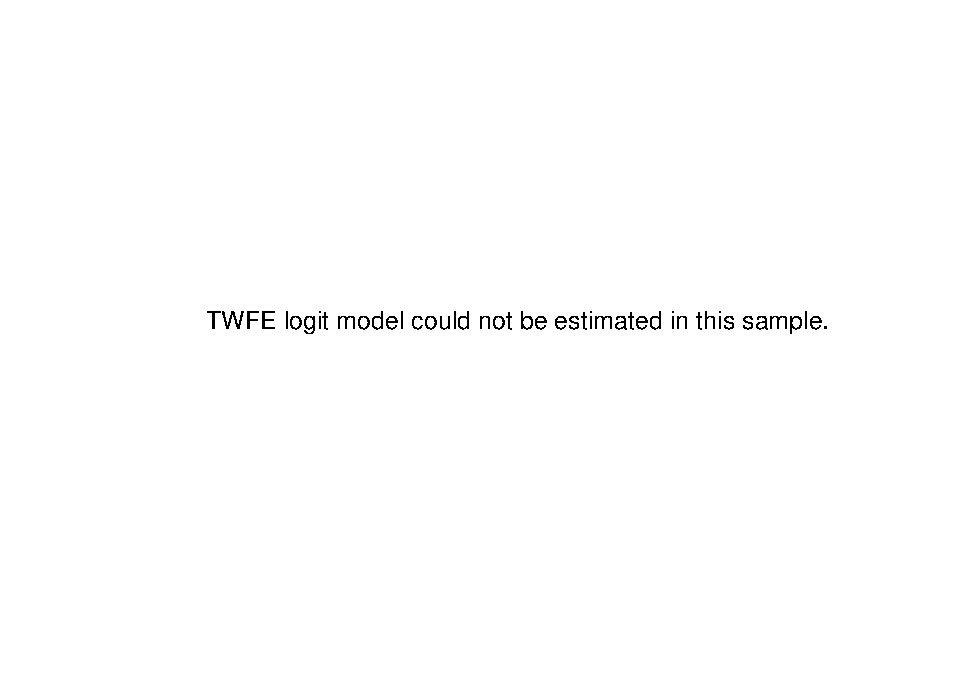
\includegraphics{Fig6_files/figure-latex/fig-event-study-aff-exit-logit-1.pdf}

\hypertarget{pooled-logit-qmle-did-with-etwfe}{%
\subsection{\texorpdfstring{Pooled logit QMLE DiD with
\texttt{etwfe}}{Pooled logit QMLE DiD with etwfe}}\label{pooled-logit-qmle-did-with-etwfe}}

\begin{itemize}
\tightlist
\item
  Following \citet{wooldridge2023simple}, we use a pooled logit QMLE DiD
  specification for the binary exit outcome.
\item
  The \texttt{etwfe} package implements the nonlinear pooled
  specification with group-level treatment timing.
\item
  This nonlinear specification is analogous to the linear ETWFE setup,
  but we avoid calling it ``ETWFE logit'' in the paper to keep the
  terminology consistent.
\end{itemize}

\hypertarget{high-income-eu}{%
\subsubsection*{High income EU}\label{high-income-eu}}
\addcontentsline{toc}{subsubsection}{High income EU}

\begin{Shaded}
\begin{Highlighting}[]
\NormalTok{es8logit }\OtherTok{\textless{}{-}}\NormalTok{ etwfe}\SpecialCharTok{::}\FunctionTok{etwfe}\NormalTok{(exitit }\SpecialCharTok{\textasciitilde{}}  \DecValTok{1}\NormalTok{  ,}
               \AttributeTok{tvar =}\NormalTok{ year, }\CommentTok{\# time var}
               \AttributeTok{gvar =}\NormalTok{ first\_year, }\CommentTok{\# group var}
               \CommentTok{\#xvar = N\_Aff\_EU  ,}
               \AttributeTok{ivar =}\NormalTok{  year }\SpecialCharTok{+}\NormalTok{ AffiliateCode, }\CommentTok{\# FEs}
               \AttributeTok{data =}\NormalTok{ aff\_highEU,}
               \AttributeTok{family =} \StringTok{"logit"}\NormalTok{,}
               \AttributeTok{vcov =} \SpecialCharTok{\textasciitilde{}}\NormalTok{country)}
\NormalTok{fixest}\SpecialCharTok{::}\FunctionTok{etable}\NormalTok{(es8logit)}
\end{Highlighting}
\end{Shaded}

\begin{verbatim}
##                                                     es8logit
## Dependent Var.:                                       exitit
##                                                             
## Constant                                  -17.57*** (0.0414)
## first_year = 2016                            0.0141 (0.1400)
## year = 2012                                15.46*** (0.0898)
## year = 2014                                16.25*** (0.1061)
## year = 2016                                16.66*** (0.1455)
## year = 2017                                16.81*** (0.1553)
## year = 2018                                16.95*** (0.1358)
## year = 2019                                17.03*** (0.1352)
## year = 2020                                17.10*** (0.1430)
## .Dtreat x first_year = 2016 x year = 2016    0.0402 (0.0635)
## .Dtreat x first_year = 2016 x year = 2017    0.0487 (0.0761)
## .Dtreat x first_year = 2016 x year = 2018    0.0170 (0.0608)
## .Dtreat x first_year = 2016 x year = 2019   0.1042. (0.0585)
## .Dtreat x first_year = 2016 x year = 2020   0.1166. (0.0662)
## ________________________________________  __________________
## S.E.: Clustered                                  by: country
## Observations                                          13,552
## Squared Cor.                                         0.09023
## Pseudo R2                                            0.10682
## BIC                                                 13,922.4
## ---
## Signif. codes: 0 '***' 0.001 '**' 0.01 '*' 0.05 '.' 0.1 ' ' 1
\end{verbatim}

\begin{Shaded}
\begin{Highlighting}[]
\CommentTok{\# イベントスタディ係数と標準誤差を抽出}
\NormalTok{coef\_vec }\OtherTok{\textless{}{-}} \FunctionTok{coef}\NormalTok{(es8logit)}
\NormalTok{se\_vec }\OtherTok{\textless{}{-}} \FunctionTok{sqrt}\NormalTok{(}\FunctionTok{diag}\NormalTok{(}\FunctionTok{vcov}\NormalTok{(es8logit)))}
\NormalTok{event\_terms }\OtherTok{\textless{}{-}} \FunctionTok{grep}\NormalTok{(}\StringTok{"\^{}}\SpecialCharTok{\textbackslash{}\textbackslash{}}\StringTok{.Dtreat:first\_year::2016:year::20(16|17|18|19|20)$"}\NormalTok{,}
                    \FunctionTok{names}\NormalTok{(coef\_vec),}
                    \AttributeTok{value =} \ConstantTok{TRUE}\NormalTok{)}

\NormalTok{es8Logit\_results }\OtherTok{\textless{}{-}} \FunctionTok{data.frame}\NormalTok{(}
  \AttributeTok{term =}\NormalTok{ event\_terms,}
  \AttributeTok{event =} \FunctionTok{as.integer}\NormalTok{(}\FunctionTok{sub}\NormalTok{(}\StringTok{".*year::"}\NormalTok{, }\StringTok{""}\NormalTok{, event\_terms)),}
  \AttributeTok{estimate =} \FunctionTok{unname}\NormalTok{(coef\_vec[event\_terms]),}
  \AttributeTok{std.error =} \FunctionTok{unname}\NormalTok{(se\_vec[event\_terms])}
\NormalTok{)}
\NormalTok{es8Logit\_results}\SpecialCharTok{$}\NormalTok{conf.low }\OtherTok{\textless{}{-}}\NormalTok{ es8Logit\_results}\SpecialCharTok{$}\NormalTok{estimate }\SpecialCharTok{{-}} \FloatTok{1.96} \SpecialCharTok{*}\NormalTok{ es8Logit\_results}\SpecialCharTok{$}\NormalTok{std.error}
\NormalTok{es8Logit\_results}\SpecialCharTok{$}\NormalTok{conf.high }\OtherTok{\textless{}{-}}\NormalTok{ es8Logit\_results}\SpecialCharTok{$}\NormalTok{estimate }\SpecialCharTok{+} \FloatTok{1.96} \SpecialCharTok{*}\NormalTok{ es8Logit\_results}\SpecialCharTok{$}\NormalTok{std.error}
\end{Highlighting}
\end{Shaded}

\hypertarget{estimation-tables}{%
\subsubsection*{Estimation tables}\label{estimation-tables}}
\addcontentsline{toc}{subsubsection}{Estimation tables}

\begin{Shaded}
\begin{Highlighting}[]
\CommentTok{\# 推定結果の係数名を表示用に整える}
\NormalTok{rename\_fn }\OtherTok{=} \ControlFlowTok{function}\NormalTok{(old\_names) \{}
\NormalTok{  new\_names }\OtherTok{=} \FunctionTok{gsub}\NormalTok{(}\StringTok{".Dtreat"}\NormalTok{, }\StringTok{"Years post treatment ="}\NormalTok{, old\_names)}
  \FunctionTok{setNames}\NormalTok{(new\_names, old\_names)}
\NormalTok{\}}

\NormalTok{models }\OtherTok{\textless{}{-}} \FunctionTok{list}\NormalTok{(}
               \StringTok{"Logit"} \OtherTok{=}\NormalTok{ es8logit)}

\FunctionTok{modelsummary}\NormalTok{(}
\NormalTok{  models, }
  \AttributeTok{shape       =}\NormalTok{ term}\SpecialCharTok{:}\NormalTok{event}\SpecialCharTok{:}\NormalTok{statistic }\SpecialCharTok{\textasciitilde{}}\NormalTok{ model, }
  \AttributeTok{coef\_rename =}\NormalTok{ rename\_fn, }\CommentTok{\# rename}
  \AttributeTok{coef\_omit =} \StringTok{".*N\_Aff*"}\NormalTok{, }
  \AttributeTok{gof\_omit    =} \StringTok{"Adj|Within|IC|RMSE"}\NormalTok{, }
  \CommentTok{\#stars       = TRUE,}
  \AttributeTok{stars =} \FunctionTok{c}\NormalTok{(}\StringTok{\textquotesingle{}*\textquotesingle{}} \OtherTok{=} \FloatTok{0.05}\NormalTok{, }\StringTok{\textquotesingle{}**\textquotesingle{}} \OtherTok{=} \FloatTok{0.01}\NormalTok{, }\StringTok{\textquotesingle{}***\textquotesingle{}} \OtherTok{=} \FloatTok{0.001}\NormalTok{) ,}
  \AttributeTok{title       =} \StringTok{"Event study (pooled logit QMLE DiD)"}\NormalTok{, }
  \AttributeTok{notes       =} \StringTok{"Std. errors are clustered at the county level"} 
\NormalTok{)}
\end{Highlighting}
\end{Shaded}

\begin{table}
\centering
\begin{talltblr}[         %% tabularray outer open
caption={Event study (pooled logit QMLE DiD)},
note{}={* p \num{< 0.05}, ** p \num{< 0.01}, *** p \num{< 0.001}},
note{ }={Std. errors are clustered at the county level},
]                     %% tabularray outer close
{                     %% tabularray inner open
colspec={Q[]Q[]},
hline{2}={1-2}{solid, black, 0.05em},
hline{30}={1-2}{solid, black, 0.05em},
hline{1}={1-2}{solid, black, 0.1em},
hline{33}={1-2}{solid, black, 0.1em},
column{2}={}{halign=c},
column{1}={}{halign=l},
}                     %% tabularray inner close
& Logit \\
(Intercept) & \num{-17.570}*** \\
& (\num{0.041}) \\
first\_year::2016 & \num{0.014} \\
& (\num{0.140}) \\
year::2012 & \num{15.455}*** \\
& (\num{0.090}) \\
year::2014 & \num{16.253}*** \\
& (\num{0.106}) \\
year::2016 & \num{16.661}*** \\
& (\num{0.146}) \\
year::2017 & \num{16.811}*** \\
& (\num{0.155}) \\
year::2018 & \num{16.950}*** \\
& (\num{0.136}) \\
year::2019 & \num{17.026}*** \\
& (\num{0.135}) \\
year::2020 & \num{17.098}*** \\
& (\num{0.143}) \\
Years post treatment =:first\_year::2016:year::2016 & \num{0.040} \\
& (\num{0.064}) \\
Years post treatment =:first\_year::2016:year::2017 & \num{0.049} \\
& (\num{0.076}) \\
Years post treatment =:first\_year::2016:year::2018 & \num{0.017} \\
& (\num{0.061}) \\
Years post treatment =:first\_year::2016:year::2019 & \num{0.104} \\
& (\num{0.058}) \\
Years post treatment =:first\_year::2016:year::2020 & \num{0.117} \\
& (\num{0.066}) \\
Num.Obs. & \num{13552} \\
R2 & \num{0.107} \\
Std.Errors & by: country \\
\end{talltblr}
\end{table}

\hypertarget{event-study-plot}{%
\subsubsection{Event study plot}\label{event-study-plot}}

\begin{Shaded}
\begin{Highlighting}[]
\CommentTok{\# イベントスタディ図}
\CommentTok{\# Add event to + 2016}
\NormalTok{es8Logit\_results}\SpecialCharTok{$}\NormalTok{event }\OtherTok{\textless{}{-}}\NormalTok{ es8Logit\_results}\SpecialCharTok{$}\NormalTok{event}

\CommentTok{\# Plot the estimate}
\NormalTok{p\_etwfe\_logit }\OtherTok{\textless{}{-}} \FunctionTok{ggplot}\NormalTok{(es8Logit\_results, }\FunctionTok{aes}\NormalTok{(}\AttributeTok{x =}\NormalTok{ event, }\AttributeTok{y =}\NormalTok{ estimate)) }\SpecialCharTok{+}
  \FunctionTok{geom\_hline}\NormalTok{(}\AttributeTok{yintercept =} \DecValTok{0}\NormalTok{) }\SpecialCharTok{+}
  \FunctionTok{labs}\NormalTok{(}\AttributeTok{x =} \StringTok{"Years post treatment"}\NormalTok{, }
       \AttributeTok{y =} \StringTok{"Effect of Brexit"}\NormalTok{,}
       \AttributeTok{title =} \StringTok{"The impacts on the exit probability"}\NormalTok{,}
       \AttributeTok{caption =} \StringTok{"Pooled logit QMLE DiD specification. Affiliate{-}level balanced panel."}
\NormalTok{       ) }\SpecialCharTok{+}
  \FunctionTok{theme\_minimal}\NormalTok{() }\SpecialCharTok{+}
  \FunctionTok{theme}\NormalTok{(}\AttributeTok{legend.position =} \StringTok{"top"}\NormalTok{) }\SpecialCharTok{+}
  \FunctionTok{geom\_text}\NormalTok{(}\FunctionTok{aes}\NormalTok{(}\AttributeTok{label =} \FunctionTok{round}\NormalTok{(estimate, }\DecValTok{3}\NormalTok{)), }
            \AttributeTok{vjust =} \SpecialCharTok{{-}}\FloatTok{0.5}\NormalTok{, }\AttributeTok{hjust =} \FloatTok{0.5}\NormalTok{, }\AttributeTok{size =} \DecValTok{3}\NormalTok{)}

\NormalTok{p\_etwfe\_logit }\OtherTok{\textless{}{-}}\NormalTok{ p\_etwfe\_logit }\SpecialCharTok{+}
  \FunctionTok{geom\_pointrange}\NormalTok{(}\FunctionTok{aes}\NormalTok{(}\AttributeTok{ymin =}\NormalTok{ conf.low, }\AttributeTok{ymax =}\NormalTok{ conf.high))}

\NormalTok{p\_etwfe\_logit}
\end{Highlighting}
\end{Shaded}

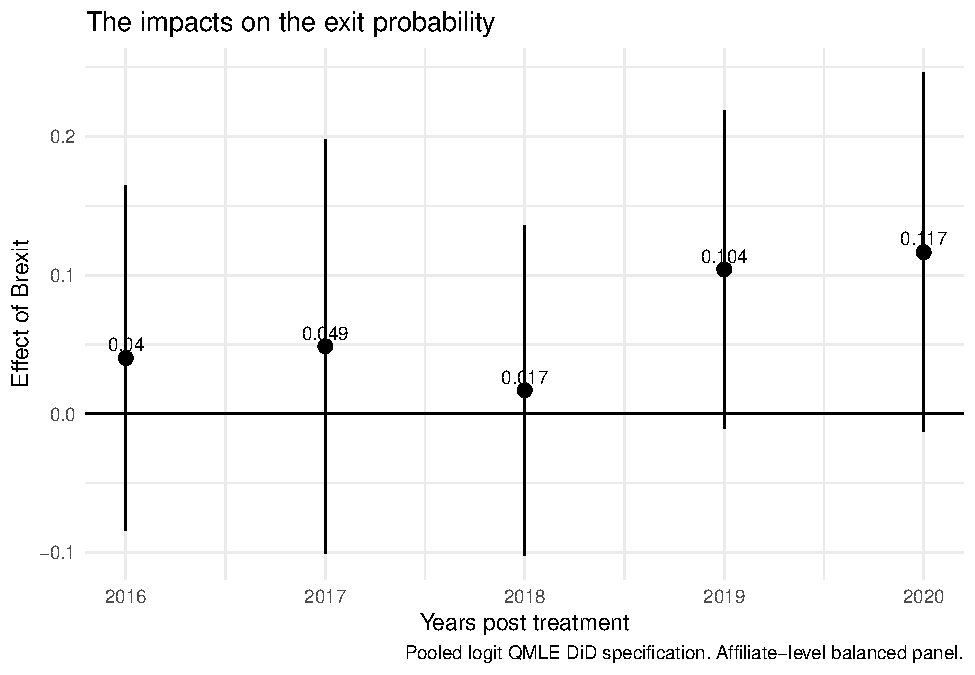
\includegraphics{Fig6_files/figure-latex/Fig6-ETWFE-exit-logit-1.pdf}

\begin{Shaded}
\begin{Highlighting}[]
\FunctionTok{ggsave}\NormalTok{(}\StringTok{"../../04\_tex/main/Fig6.eps"}\NormalTok{, }\AttributeTok{dpi =} \DecValTok{300}\NormalTok{)}
\end{Highlighting}
\end{Shaded}

\hypertarget{ux30d7ux30ecux30c8ux30ecux30f3ux30c9ux691cux5b9a}{%
\subsection{プレトレンド検定}\label{ux30d7ux30ecux30c8ux30ecux30f3ux30c9ux691cux5b9a}}

\hypertarget{all-observations}{%
\subsubsection*{All observations}\label{all-observations}}
\addcontentsline{toc}{subsubsection}{All observations}

\begin{Shaded}
\begin{Highlighting}[]
\CommentTok{\# 事前係数をまとめたプレトレンド検定}

\NormalTok{es10 }\OtherTok{\textless{}{-}}\NormalTok{ fixest}\SpecialCharTok{::}\FunctionTok{feglm}\NormalTok{(exitit }\SpecialCharTok{\textasciitilde{}} \DecValTok{1}\SpecialCharTok{+} \FunctionTok{i}\NormalTok{(year, GBR, }\DecValTok{2014}\NormalTok{) }
                       \SpecialCharTok{|}\NormalTok{ year }\SpecialCharTok{+}\NormalTok{ GBR, }
               \AttributeTok{data =}\NormalTok{ aff\_highEU,}
               \CommentTok{\#family = binomial(link = "logit"),}
               \AttributeTok{family =} \StringTok{"logit"}\NormalTok{,}
               \AttributeTok{vcov =} \SpecialCharTok{\textasciitilde{}}\NormalTok{ country)}
\NormalTok{fixest}\SpecialCharTok{::}\FunctionTok{etable}\NormalTok{(es10)}
\end{Highlighting}
\end{Shaded}

\begin{verbatim}
##                               es10
## Dependent Var.:             exitit
##                                   
## GBR x year = 2012 -0.0027 (0.0568)
## GBR x year = 2016  0.0392 (0.0603)
## GBR x year = 2017  0.0477 (0.0740)
## GBR x year = 2018  0.0160 (0.0619)
## GBR x year = 2019 0.1032. (0.0593)
## GBR x year = 2020  0.1156 (0.0704)
## Fixed-Effects:    ----------------
## year                           Yes
## GBR                            Yes
## _________________ ________________
## S.E.: Clustered        by: country
## Observations                11,858
## Squared Cor.               0.04301
## Pseudo R2                  0.03921
## BIC                       13,920.5
## ---
## Signif. codes: 0 '***' 0.001 '**' 0.01 '*' 0.05 '.' 0.1 ' ' 1
\end{verbatim}

\begin{Shaded}
\begin{Highlighting}[]
\NormalTok{fixest}\SpecialCharTok{::}\FunctionTok{iplot}\NormalTok{(es10, }\AttributeTok{pt.join =} \ConstantTok{TRUE}\NormalTok{,}
      \AttributeTok{main =} \StringTok{"Effect of Brexit on exit probability"}\NormalTok{,}
      \AttributeTok{sub =} \StringTok{"Affiliate{-}level balanced panel"}\NormalTok{,}
      \AttributeTok{xlab =} \StringTok{"Logit model"}
\NormalTok{      )}
\end{Highlighting}
\end{Shaded}

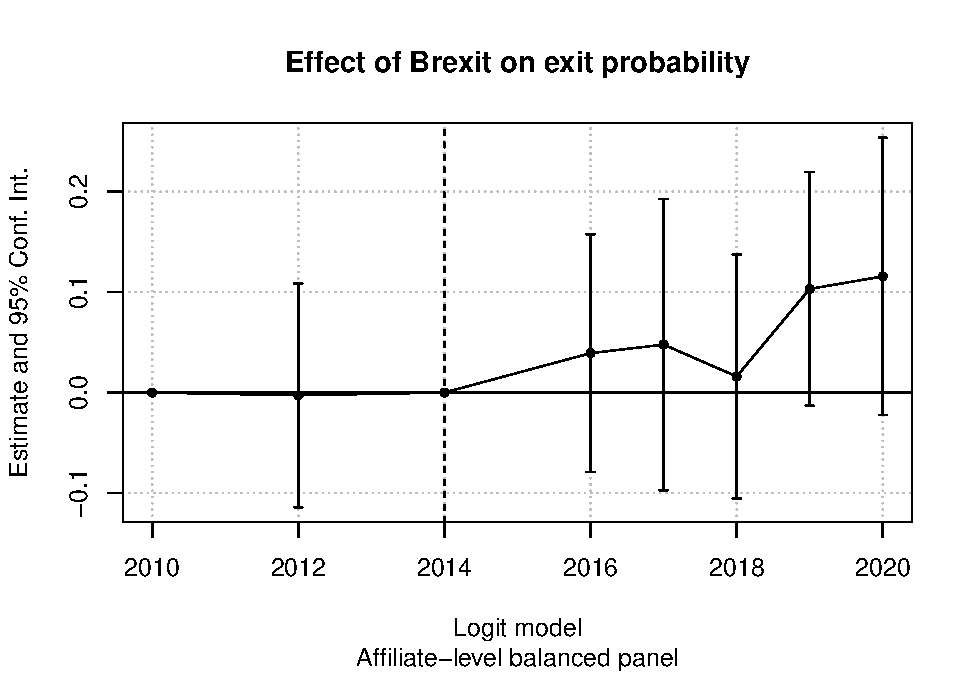
\includegraphics{Fig6_files/figure-latex/event-study-test1-1.pdf}

\hypertarget{not-yet-treated-observations}{%
\subsubsection*{Not-yet treated
observations}\label{not-yet-treated-observations}}
\addcontentsline{toc}{subsubsection}{Not-yet treated observations}

\begin{Shaded}
\begin{Highlighting}[]
\CommentTok{\# Subset of year \textless{}=2014}
\NormalTok{aff\_highEU\_pre2014 }\OtherTok{\textless{}{-}}\NormalTok{ aff\_highEU }\SpecialCharTok{\%\textgreater{}\%} \FunctionTok{filter}\NormalTok{(year }\SpecialCharTok{\textless{}=} \DecValTok{2014}\NormalTok{)}

\CommentTok{\# Fixed effects \& Interaction terms}
\NormalTok{aff\_highEU\_pre2014}\SpecialCharTok{$}\NormalTok{year2010 }\OtherTok{\textless{}{-}} \FunctionTok{ifelse}\NormalTok{(aff\_highEU\_pre2014}\SpecialCharTok{$}\NormalTok{year }\SpecialCharTok{==} \DecValTok{2010}\NormalTok{, }\DecValTok{1}\NormalTok{, }\DecValTok{0}\NormalTok{)}
\NormalTok{aff\_highEU\_pre2014}\SpecialCharTok{$}\NormalTok{year2012 }\OtherTok{\textless{}{-}} \FunctionTok{ifelse}\NormalTok{(aff\_highEU\_pre2014}\SpecialCharTok{$}\NormalTok{year }\SpecialCharTok{==} \DecValTok{2012}\NormalTok{, }\DecValTok{1}\NormalTok{, }\DecValTok{0}\NormalTok{)}
\NormalTok{aff\_highEU\_pre2014}\SpecialCharTok{$}\NormalTok{year2014 }\OtherTok{\textless{}{-}} \FunctionTok{ifelse}\NormalTok{(aff\_highEU\_pre2014}\SpecialCharTok{$}\NormalTok{year }\SpecialCharTok{==} \DecValTok{2014}\NormalTok{, }\DecValTok{1}\NormalTok{, }\DecValTok{0}\NormalTok{)}
\NormalTok{aff\_highEU\_pre2014}\SpecialCharTok{$}\NormalTok{year2010GBR }\OtherTok{\textless{}{-}}\NormalTok{ aff\_highEU\_pre2014}\SpecialCharTok{$}\NormalTok{year2010 }\SpecialCharTok{*}\NormalTok{ aff\_highEU\_pre2014}\SpecialCharTok{$}\NormalTok{GBR}
\NormalTok{aff\_highEU\_pre2014}\SpecialCharTok{$}\NormalTok{year2012GBR }\OtherTok{\textless{}{-}}\NormalTok{ aff\_highEU\_pre2014}\SpecialCharTok{$}\NormalTok{year2012 }\SpecialCharTok{*}\NormalTok{ aff\_highEU\_pre2014}\SpecialCharTok{$}\NormalTok{GBR}
\NormalTok{aff\_highEU\_pre2014}\SpecialCharTok{$}\NormalTok{year2014GBR }\OtherTok{\textless{}{-}}\NormalTok{ aff\_highEU\_pre2014}\SpecialCharTok{$}\NormalTok{year2014 }\SpecialCharTok{*}\NormalTok{ aff\_highEU\_pre2014}\SpecialCharTok{$}\NormalTok{GBR}


\NormalTok{es11 }\OtherTok{\textless{}{-}}\NormalTok{ fixest}\SpecialCharTok{::}\FunctionTok{feglm}\NormalTok{(exitit }\SpecialCharTok{\textasciitilde{}}\NormalTok{  year2010GBR }\SpecialCharTok{+}\NormalTok{ year2012GBR }\SpecialCharTok{+}\NormalTok{ year2014GBR}
                       \SpecialCharTok{|}\NormalTok{ year , }
               \AttributeTok{data =}\NormalTok{ aff\_highEU\_pre2014,}
               \CommentTok{\#family = binomial(link = "logit"),}
               \AttributeTok{family =} \StringTok{"logit"}\NormalTok{,}
               \AttributeTok{vcov =} \SpecialCharTok{\textasciitilde{}}\NormalTok{ country)}
\NormalTok{fixest}\SpecialCharTok{::}\FunctionTok{etable}\NormalTok{(es11)}
\end{Highlighting}
\end{Shaded}

\begin{verbatim}
##                            es11
## Dependent Var.:          exitit
##                                
## year2012GBR     0.0123 (0.1276)
## year2014GBR     0.0151 (0.1506)
## Fixed-Effects:  ---------------
## year                        Yes
## _______________ _______________
## S.E.: Clustered     by: country
## Observations              3,388
## Squared Cor.            0.02009
## Pseudo R2               0.02320
## BIC                     2,942.3
## ---
## Signif. codes: 0 '***' 0.001 '**' 0.01 '*' 0.05 '.' 0.1 ' ' 1
\end{verbatim}

\begin{Shaded}
\begin{Highlighting}[]
\CommentTok{\# Joint Wald test of the coefficients}
\CommentTok{\# https://lrberge.github.io/fixest/reference/wald.html\#ref{-}examples}
\NormalTok{fixest}\SpecialCharTok{::}\FunctionTok{wald}\NormalTok{(es11, }
             \AttributeTok{keep =} \StringTok{"year201[[:digit:]]GBR"}\NormalTok{, }\CommentTok{\# Regular expression}
             \AttributeTok{print =} \ConstantTok{TRUE}\NormalTok{)}
\end{Highlighting}
\end{Shaded}

\begin{verbatim}
## Wald test, H0: joint nullity of year2012GBR and year2014GBR
##  stat = 0.005064, p-value = 0.994949, on 2 and 3,384 DoF, VCOV: Clustered (country).
\end{verbatim}

\begin{Shaded}
\begin{Highlighting}[]
\CommentTok{\# Coefplot }
\NormalTok{fixest}\SpecialCharTok{::}\FunctionTok{coefplot}\NormalTok{(es11, }
                 \AttributeTok{keep =} \StringTok{"year201[[:digit:]]GBR"}\NormalTok{,}
                 \AttributeTok{main =} \StringTok{"Event study test"}\NormalTok{,}
                 \AttributeTok{sub =} \StringTok{"Affiliate{-}level balanced panel"}\NormalTok{,}
                 \AttributeTok{xlab =} \StringTok{"Logit model"}
\NormalTok{                 )}
\end{Highlighting}
\end{Shaded}

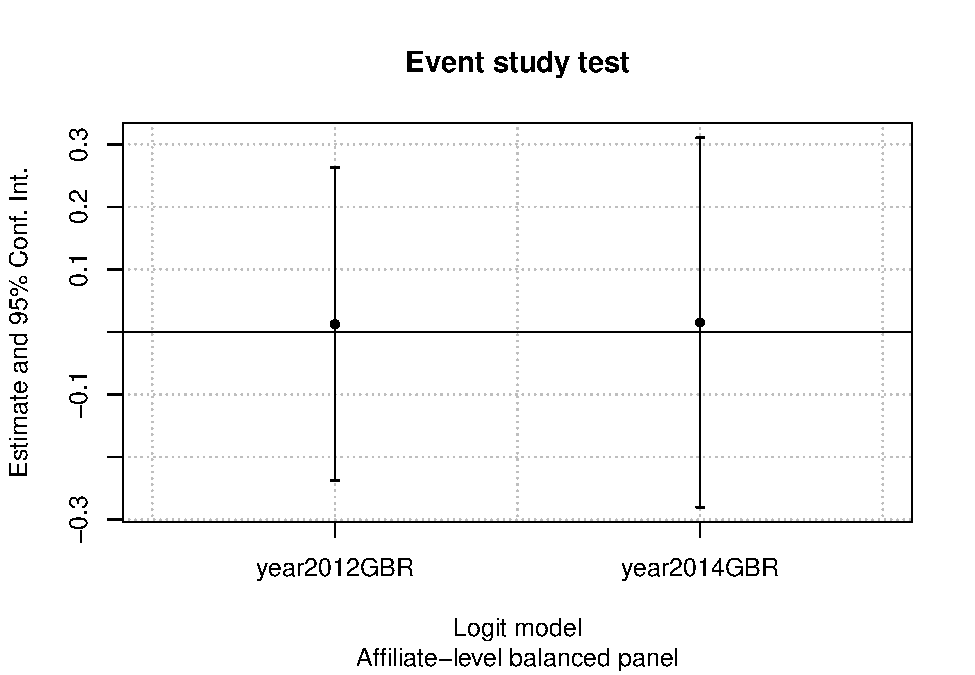
\includegraphics{Fig6_files/figure-latex/event-study-test2-1.pdf}

\hypertarget{references}{%
\section*{References}\label{references}}
\addcontentsline{toc}{section}{References}

\begin{itemize}
\item
  \href{https://tilburgsciencehub.com/topics/visualization/reporting-tables/reportingtables/kableextra/}{Create
  a publication-ready LaTeX regression table with \texttt{kableExtra} in
  R}
\item
  \href{https://modelsummary.com/articles/modelsummary.html}{modelsummary:
  regression tables}
\item
  \href{https://lrberge.github.io/fixest/articles/exporting_tables.html\#exporting-multiple-estimations-to-latex}{fixest:
  Exporting estimation tables}
\end{itemize}

For fixest: -
\href{https://cran.r-project.org/web/packages/fixest/vignettes/fixest_walkthrough.html}{Fast
Fixed-Effects Estimation: Short Introduction}

For OLS: -
\href{https://lrberge.github.io/fixest/reference/feols.html}{Fixed-effects
OLS estimations}

For Logit model: -
\href{https://lrberge.github.io/fixest/reference/feglm.html}{Fixed-effects
GLM estimations} - \href{https://rdrr.io/r/stats/family.html}{family:
Family Objects for Models} -
\href{https://stats.oarc.ucla.edu/r/dae/logit-regression/}{LOGIT
REGRESSION \textbar{} R DATA ANALYSIS EXAMPLES}

\end{document}
